\documentclass{article}

\usepackage[brazil]{babel}
\usepackage[T1]{fontenc}
\usepackage[a4paper, margin=1.5cm]{geometry}
\usepackage[colorlinks, urlcolor=blue, citecolor=red]{hyperref}
\usepackage[utf8]{inputenc}
\usepackage{amsmath, graphicx}

\title{\textbf{Utilizando redes neurais para identificar dígitos manuscritos}}
\author{Emmanuel Podestá Jr., Gustavo Zambonin\thanks{
        \texttt{\{emmanuel.podesta,gustavo.zambonin\}@grad.ufsc.br} \hfill
        \texttt{\href{https://github.com/zambonin/ufsc-ine5430}{src/}}
    } \\
    \small{Inteligência Artificial (UFSC -- INE5430)}
}
\date{}

\begin{document}

\maketitle

\section{Fundamentação}

A utilização de redes neurais para processamento de imagens é bastante conhecida
na literatura. Neste trabalho, uma implementação em Python 3 a partir da
biblioteca \href{http://pybrain.org/}{PyBrain} demonstra a capacidade de
reconhecimento de padrões desta abordagem computacional. \medskip

O conjunto escolhido para classificação consiste de uma fração da base de dados
\href{http://yann.lecun.com/exdb/mnist/}{MNIST} (\emph{Mixed National Institute
of Standards and Technology database}), organizada como uma lista de imagens,
cada qual como uma lista de \emph{pixels} no intervalo $[-1, 1]$ e um valor
inteiro representando o dígito correspondente no intervalo $[1, 10]$. A
normalização das intensidades de preto é realizada apenas caso a visualização
das imagens seja desejada; o método \emph{feature scaling} é aplicado a cada uma
das listas para que uma imagem no formato PGM \emph{{Portable Graymap Format}})
seja gerada.

\begin{figure}[htbp]
    \[ x' = \frac{(x - min(y)) \times 255}{max(y) - min(y)} \] \vspace{-5mm}
    \caption{Equação que normaliza valores para o intervalo $[0, 255]$. A
    lista de valores original é representada por $y$, $x$ é valor atual
    e $x'$ é o valor normalizado.}
\end{figure}

Do contrário, é necessário apenas adaptar os dígitos correspondentes à
identidade das imagens para vetores de tamanho $10$ (pois existem $10$ dígitos
diferentes) com apenas uma coordenada ativa, aquela cujo índice é igual ao seu
valor módulo 10. A arquitetura da rede neural é baseada nesta organização de
dados; três camadas são criadas para processar os dígitos:

\begin{itemize}
    \item a camada de entrada é construída com 400 neurônios, o número de
        \emph{pixels} de uma dada imagem; observou-se que não é necessário
        utilizar uma função complexa de processamento de valores, bastando
        apenas uma função de ativação linear ($f(x) = x$).

    \item a camada ``escondida'', construída com 40 neurônios, utilizará da
        função de ativação tangente hiperbólica para atualizar seus valores
        ($f(x) = \frac{2}{1 + e^{-2x}} -1$).

    \item a camada de saída, construída com 10 neurônios, o número de possíveis
        saídas, classificará o resultado atual a partir da função
        \emph{softmax}, que transforma um vetor $\mathbf{z}$ com valores reais
        arbitrários para um vetor $\sigma(\mathbf{z})$ com valores reais no
        intervalo $(0, 1)$, cuja soma é $1$. Ambos os vetores têm dimensão $K$.
        A saída dessa função pode ser utilizada para representar uma
        distribuição de probabilidades sobre $K$ diferentes possibilidades,
        relevante no contexto de classificação de dados.
        \begin{align*}
            \sigma(\mathbf{z})_j = \frac{e^{z_j}}{\sum_{k=1}^K e^{z_k}}
            \; \forall j = 1, \ldots, K
        \end{align*}
\end{itemize}

\section{Implementação}

A separação dos dados em bases de treino e de teste, sob uma proporção 80/20,
foi feita após embaralhamento das imagens na lista. O treinador escolhido
utiliza o método do gradiente descendente com mini-\emph{batches} e
\emph{backpropagation}, com taxa de aprendizado $\mu = 0.04$ e treino por $30$
épocas. Estudando o problema, percebeu-se que com estes parâmetros, os
resultados são razoáveis, apresentando uma porcentagem de acertos interessante
($\approx 98\%$ considerando toda a base de dados fornecida), sem muita
flutuação ou estagnação de valores; um número muito maior de épocas torna o
desempenho proibitivamente baixo. \medskip

O programa responsável por controlar a rede neural pode ser encontrado em
\texttt{mnist\_classify.py}. Um exemplo de execução segue abaixo; o argumento
\texttt{--plot} gera a matriz de confusão apresentada em seguida.

\begin{verbatim}
    $ python mnist_classify.py --plot
    Epoch:   1   All: 81.74%   Train: 82.75%   Test: 77.70%
    Epoch:   2   All: 87.16%   Train: 87.92%   Test: 84.10%
    Epoch:   3   All: 89.88%   Train: 90.72%   Test: 86.50%
    ...
    Epoch:  28   All: 97.76%   Train: 99.95%   Test: 89.00%
    Epoch:  29   All: 97.90%   Train: 99.95%   Test: 89.70%
    Epoch:  30   All: 97.92%   Train: 99.95%   Test: 89.80%
\end{verbatim}

\begin{figure}[htbp]
    \centering
    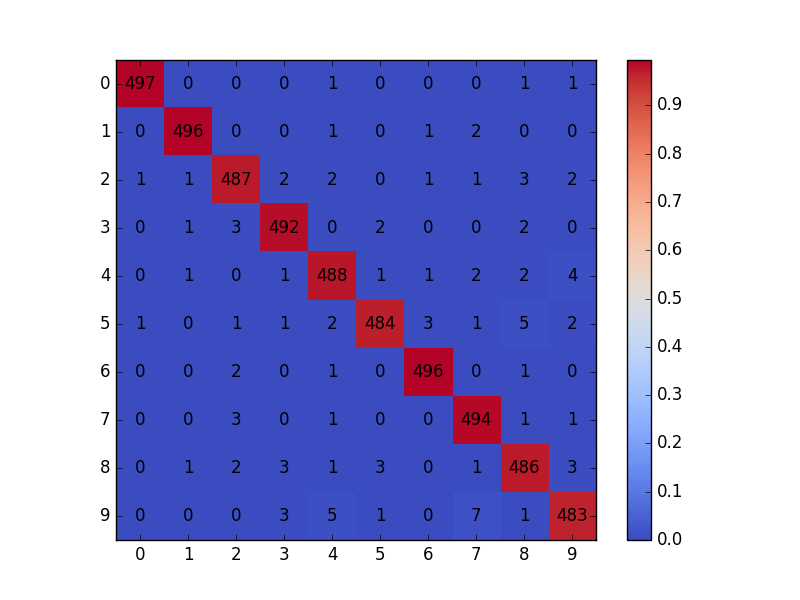
\includegraphics[scale=0.65]{confusion_matrix}
    \caption{Matriz de confusão gerada após a finalização do treinamento
        com o conjunto de argumentos padrão.}
    \label{fig01}
\end{figure}

\end{document}
